\subsection{Nonparametric density modeling with a transformed Gaussian process}
Our next application is the Gaussian process density sampler of~\cite{adams_gpds},
%This finds application in Bayesian density modeling applications, where one wishes to place 
a nonparametric prior for probability densities induced by a logistic transformation of a random function from a Gaussian process.  
Letting $\sigma(\cdot)$ denote the logistic function, the random density is 
%$$p(x) \propto g(x) \sigma\{ f(x) \},\quad 
%f \sim \mbox{\small{GP}}, $$
\begin{align}
g(x) &\propto g_0(x) \sigma\{f(x)\},\qquad
f \sim  \mbox{\small{GP}}, \nonumber 
\end{align}
with $g_0(\cdot)$ a parametric base density and $\mbox{\small{GP}}$ denoting a Gaussian process.
%However, %the fact that the sigmoid is bounded above by $1$ gives us 
The inequality
%\begin{align}
$g_0(x) \sigma\{f(x)\} \le g_0(x)$
%\end{align}
allows a rejection sampling algorithm %where we draw perfect samples by successively 
by making proposals from $g_0(\cdot)$.
%can do this sequentially, sampling a new 
At a proposed location $x^*$, we sample the function value $f(x^*)$ conditioning on 
all previous evaluations, and accept the proposal with probability 
$\sigma\{f(x^*)\}$.  Such a scheme involves no approximation error, and only requires evaluating the random function on a finite set of points.
Algorithm \ref{alg:gpds} describes the steps involved in generating $n$ observations.

{
\begin{algo}
{Generate $n$ new samples from the Gaussian process density sampler}\label{alg:gpds}
\begin{itemize}
  \item[]
\begin{tabular}{p{.9cm}p{12.2cm}}
{Input:}  & A base probability density $g_0(\cdot)$. \\
                 & Previous accepted and rejected proposals $\tilde{X}$ and $\tilde{Y}$. \\
                 & Gaussian process evaluations $f_{\tilde{X}}$ and $f_{\tilde{Y}}$ at these locations. \\
{Output:} & $n$ new samples $X$, with the associated rejected proposals $Y$. \\ % from the random density $p(\cdot)$.  \\
                 & Gaussian process evaluations $f_X$ and $f_Y$ at these locations. \\
\end{tabular}
\vspace*{-8pt}
\begin{tabbing}
  \enspace Repeat \\
  \qquad Sample a proposal $y$ from $g_0(\cdot)$. \\
  \qquad Sample $f_y$, the Gaussian process evaluated at $y$, conditioning on $f_X$, $f_Y$, $f_{\tilde{X}}$ and $f_{\tilde{Y}}$. \\ % at $X$ and $Y$  %, and the covariance kernel $\mathcal{K}$.
  \qquad {With probability }{$\sigma(f_y)$} \\
  \qquad \qquad Accept $y$ and add it to $X$. Add $f_y$ to $f_X$.\\
  \qquad  {Else} \\
  \qquad  \qquad Reject $y$ and add it to $Y$. Add $f_y$ to $f_Y$.\\
  \enspace Until {$n$ samples are accepted}.
\end{tabbing}
\end{itemize}
\end{algo}
}



\subsection{Posterior inference}
% The GPDS defines a nonparametric prior over probability densities on $\mathbb{X}$. 
Given observations $X = \{x_1, \ldots, x_n\}$,
we are interested in $p(g\mid X)$, the posterior over the underlying density. %, or equivalently, % $p(\cdot)$. 
Since $g$ is determined by the modulating function $f$, we focus on %there is a one-to-one mapping between the density and the 
%function $f(\cdot)$, we focus on 
$p(f\mid X)$. %By itself, this is a complicated quantity, and 
While this quantity is doubly intractable,
after augmenting the state space to include the proposals $\cY$ from the rejection sampling algorithm, %of the previous section results in a much simpler probability distribution. 
%In particular, 
 $p(f\mid X,\cY)$ has density $\prod_{i=1}^n \sigma\left\{f(x_i)\right\} \prod_{i=1}^{|\cY|} \left[1-\sigma\left\{f(y_i)\right\}\right]$
  with respect to the Gaussian process prior; see also~\cite{adams_gpds}.
In words, the posterior over $f$ evaluated at $X \cup \cY$ is just the posterior from a Gaussian process
classification problem with a logistic link-function, and with the accepted and rejected proposals corresponding to the two classes.
%x_i &\sim p(x) \qquad i = 1, \cdots, n
Markov chain Monte Carlo methods such as Hamiltonian Monte Carlo or elliptical slice sampling~\citep{murray2010} 
are applicable in such a situation. Given $f$ on $X \cup \cY$, the Gaussian process can be evaluated anywhere else by 
conditionally sampling from a multivariate normal.

%The question then is how to 
Sampling the rejected proposals $\cY$ given $X$ and $f$ is straightforward by Algorithm \ref{prop:rej_post}:
run the rejection sampler until $n$ accepts, and treat the rejected proposals generated
along the way as $\cY$. In practice, we do not have access to the entire function $f$, only its
values evaluated on $X$ and $\cY_{old}$, the locations of the previous thinned variables. However, just as under the generative 
mechanism, we can retrospectively evaluate the function $f$ where needed.
After proposing from $g_0(\cdot)$, we sample the value of the function at this location conditioned on all previous evaluations, and
use this value to decide whether to accept or reject. We outline the inference algorithm in
Algorithm \ref{alg:gpds_mcmc}, noting that it is much simpler than that proposed in~\cite{adams_gpds}.
We also refer to that paper for limitations of the exchange sampler in this problem.

  \begin{figure}
  \centering
    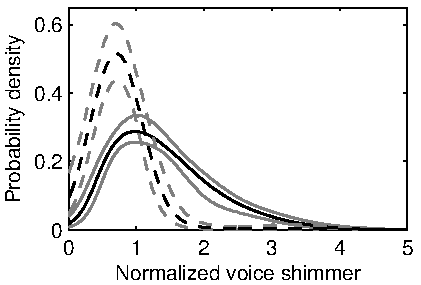
\includegraphics[width=.35\textwidth]{figs/plot_parkinson_new.pdf}
    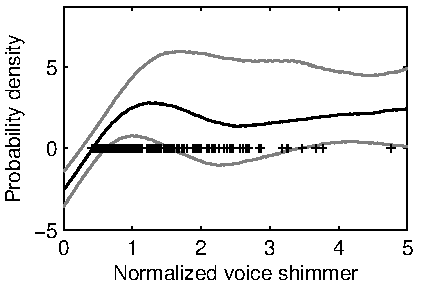
\includegraphics[width=.35\textwidth]{figs/plot_parkinson_int_new.pdf}
\caption{Inferences for the Parkinson's dataset: (left) posterior density for positive/control groups, shown as 
solid/ dashed lines, (right) posterior distribution of the Gaussian process function for
positive group with observations. Both panels show the median with $80$ percent credible intervals.}
  \label{fig:plot_glx}
  \end{figure}
{
\begin{algo}{A Markov chain iteration for inference in the Gaussian process density sampler}\label{alg:gpds_mcmc}
  \begin{itemize}
    \item[]
\begin{tabular}{p{.9cm}p{12.2cm}}
{Input:}  & Observations $X$ with corresponding function evaluations $\tilde{f}_X$. \\
          & Current rejected proposals $\tilde{Y}$ with corresponding function evaluations $\tilde{f}_{\tilde{Y}}$. \\
{Output:} & New rejected proposals $Y$. \\ % from the random density $p(\cdot)$.  \\
                 & New Gaussian process evaluations $f_X$ and $f_Y$ at $X$ and $Y$. \\
                 & New hyperparameters. \\
\end{tabular}
\begin{tabbing}
  \enspace Run Algorithm \ref{alg:gpds} to produce $|X|$ accepted samples, with $X, \tilde{Y}, \tilde{f}_X$ and $\tilde{f}_{\tilde{Y}}$ as inputs. \\
  \enspace Replace $\tilde{Y}$ and $f_{\tilde{Y}}$ with values returned by the previous step; call these $Y$ and $\hat{f}_Y$.\\
  \enspace Update $\tilde{f}_X$ and $\hat{f}_Y$ using for example, hybrid Monte Carlo, to get $f_X$ and $f_Y$.\\
  \enspace Update Gaussian process and base-distribution hyperparameters.
\end{tabbing}
  \end{itemize}
\end{algo}
}


\subsection{Experiments}   \label{sec:gpds_expt}

  Voice changes are a symptom and measure of onset of Parkinson's disease, and one attribute is voice shimmer, a measure of variation in
  amplitude. We consider a dataset of such measurements for subjects with and without the disease~\citep{little07}, with
%Voice-shimmer is a measure of variation in amplitude, and there are 
147 measurements with, and 48 without the disease.
We normalized these to vary from $0$ to $5$, and  used the model of~\cite{adams_gpds} as a prior on the underlying probability densities. 
We set $g_0(\cdot)$ to a normal $\mathcal{N}(\mu,\sigma^2)$, 
with a normal-inverse-Gamma prior on $(\mu, \sigma)$. The latter had its mean, inverse-scale, degrees-of-freedom and variance
set to $0,.1,1$ and $10$. The Gaussian process had a 
squared-exponential kernel, with variance and length-scale of $1$.
For each case, we ran a Matlab implementation of our data augmentation algorithm to produce 2,000 posterior samples after a burn-in of $500$ samples. 

  \begin{figure}
  \centering
    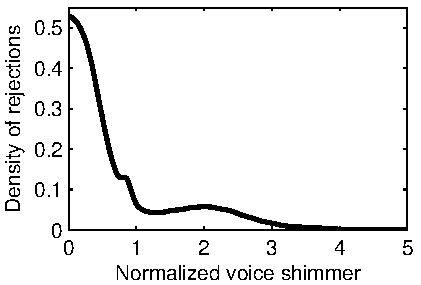
\includegraphics[width=.35\textwidth]{figs/plot_park_thin.pdf}
    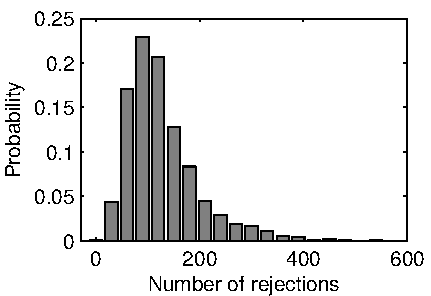
\includegraphics[width=.35\textwidth]{figs/plot_park_thin2.pdf}
\caption{Rejected proposals for the Parkinson's dataset: (left) kernel density estimate of locations of rejected proposals, and (right) histogram of 
the number of rejected proposals for the positive group.}
  \label{fig:plot_glx2}
  \end{figure}


  The left panel in Figure~\ref{fig:plot_glx} shows the resulting posterior over densities, corresponding to $\theta$ in Algorithm~\ref{alg:rej_post}.
The control group is fairly Gaussian, while the disease group is skewed to the right.
%This is clearly multimodal and non-Gaussian, with the modulating function allowing low-probability areas around either side of the main cluster
%of observations. The right bump away from the origin is slightly thinner that the left one because we have fewer observations there, but also
%since we centered our model around the origin.
The right panel focuses on the deviation from normality by plotting the posterior over the latent function $f$. 
%Outside the interval $[0,10]$, this reverts to the prior, with the decaying tails of the base-measure $g_0(\cdot)$ accounting for the lack of observations there. 
%Inside the interval $[0,10]$, there are two dips in the Gaussian process intensity at $[1,3]$
%and $[7,9]$, while over $[3,7]$, it 
We see that to the right of $0.5$, this deviation is larger than its prior mean of zero, implying larger probability than under a Gaussian density.
Figure~\ref{fig:plot_glx2} studies the distribution of the rejected proposals $\cY$.
The left plot shows the distribution of their locations:
most of these occured near the origin. Here, the disease density reverts to Gaussian or even sub-Gaussian density, with the intensity function taking small 
values.  The right plot is a histogram of the number of rejected proposals: this is typically 
around 100 to 150, though
the largest value we observed was $668$. Since inference on the latent function involves evaluating it at the accepted as
well as rejected proposals, the largest covariance matrix we had to deal with was about $600 \times 600$; typical values were around $100 \times 100$. Using
the same setup as Section~\ref{sec:Bayes_expt}, it took a na\"ive Matlab implementation 26 and 18 minutes to run 2,500 iterations for the
disease and control datasets. One can imagine 
computations becoming unwieldy for a large number of observations, or when there is large mismatch between the true density and the base-measure $g_0(\cdot)$. 
In such situations, one might have to choose the Gaussian process covariance kernel more carefully, use one of many sparse approximation techniques,
or use other nonparametric priors like splines instead. In all these cases, we can use our algorithm to recover the rejected proposals $\cY$, 
and given these, posterior inference for $f$ 
can be carried out using standard techniques.
%, this effect
%vanishes when we place a more uniformative prior on the parameters of $g_0(\cdot)$.

